\documentclass[a4paper,oneside,onecolumn,article,draft]{memoir}
\counterwithout{section}{chapter}

\usepackage[T1]{fontenc}
\usepackage[utf8]{inputenc}
\usepackage{kpfonts}

\usepackage{textgreek}

\usepackage[final]{graphicx}

%% remove colorlinks option when ready for print
\usepackage[final,hyperindex,hyperfootnotes,bookmarksnumbered,colorlinks]{hyperref}

\usepackage{amsmath}

\newsubfloat{figure} % allow subfigures

\usepackage[textsize=footnotesize]{todonotes}
%% new command for box about missing references
\newcommand{\addref}[1]{\todo[color=red!40,size=\tiny]{Add reference: #1}}

\usepackage{tikz}

\usepackage[sectionbib,round,comma]{natbib}
\bibliographystyle{agu}

\usepackage{siunitx}
\DeclareSIUnit{\bp}{bp} % base pairs
\newcommand{\pcent}[1]{\SI{#1}{\percent}}
\newcommand{\dc}[1]{\SI{#1}{\degreeCelsius}}

\newcommand{\captionIntro}[2]{\caption[#1]{\textbf{#1} #2}}

%% Just like we have cite and citep to cite in text and between parentheses,
%% have the same for fref, tref, etc...
\newcommand{\frefp}[1]{(\fref{#1})}
\newcommand{\Srefp}[1]{(\Sref{#1})}

\newcommand{\species}[1]{\textit{#1}}
\newcommand{\command}[1]{\texttt{#1}}

%% NCBI Style Guide, Chapter 5 "Style Points and Conventions", recommends
%% italic for gene names (except in long list of genes), and roman for
%% protein names.
\newcommand{\gene}[1]{\textit{#1}}
\newcommand{\protein}[1]{#1}

\newcommand{\Kon}{$K_{on}$}
\newcommand{\Koff}{$K_{off}$}
\newcommand{\halflife}[1][]{$t_{1/2}$#1}

\newcommand{\G}[1]{G$_#1$}  % for G0, G1, and G2 phases


\author{David Miguel Susano Pinto \and Kevin F. Sullivan \and Andrew Flaus}
\title{Application of FRAP to histones in human cell nuclei}

\begin{document}

  \maketitle

  \begin{abstract}
    \todo{Rewrite after body is completed}
    To further the understanding of nucleosome structure and positioning
    in DNA, we aim to measure kinetic differences between wild type and
    mutant histones in live cells. Fluorescent Recovery After Photobleaching
    is a technique successfully used before to show the different kinetics and
    populations between different histone types. Using the same approach with
    our most disrupting histone mutant, we test the limits of FRAP when
    faced with extremely slow exchange ratios.
  \end{abstract}

  \section{Introduction}

  \subsection{Histones contribute to nucleosome dynamics}

<<<<<<< HEAD
    The chromatin packaging of eukaryote genomes performs the functions of
    compacting very large lengths of DNA into the microscopic cell nucleus,
    facilitating chromosomal movements during cell division,
    and acting as a substrate for molecular mechanisms acting on the genome.

    The building block of eukaryotic chromatin structure is the nucleosome, 
    comprising \SI{147}{\bp} of DNA wrapped around an octamer of two copies each
    of core histones H2A, H2B, H3 and H4 \citep{luger1997crystal}.
    Nucleosome core particles are arranged in a linear chain separated by DNA linkers,
    and can be further compacted into higher order chromatin structures.

    Chromatin functions at both the molecular and cellular levels 
    requires the capability for dynamic rearrangement.
    Chromatin structure can be modulated through nucleosomes
    by changing the arrangement of histones and DNA in a process known as remodelling \addref{?},
    or by altering histone chemical composition 
    through post-translational modification \addref{?} or exchange of histone variants \addref{?}.

    A large amount of evidence has been accumulated about 
    the static structure of the nucleosome at atomic resolution \addref{?},
    and about the static arrangement of polymeric chromatin \addref{?}.
    However, the mechanisms for dynamic rearrangement of chromatin
    are much less well understood or integrated between the molecular and polymer levels \addref{?}.

  \subsection{Nucleosome dynamics and histone SIN mutants}

    The archetype of ATP-dependent nucleosome remodelling enzymes is the SWI/SNF complex,
    which was identified in screens for mating type SWItching \citep{SWI-mutants}
    and Sucrose Non Fermentation \citep{SNF-mutants-original-discovery, SNF-mutants2}
    in \textit{Saccharomyces cerevisiae}.

    Mutations were subsequently identified that compensate for the loss of the SWI/SNF complex
    that are collectively known as SIN mutations because they provide SWI/SNF INdependence \addref{?}.
    A subset of SIN mutants are single amino-acid changes in core histones H3 and H4,
    providing a direct link between SWI/SNF and chromatin.
    This also suggests the mutated residues in the histone proteins 
    influence the same pathways for nucleosome dynamics leveraged by the enzyme 
    and that these residues are significant for nucleosome stability.

    This predicted that the stability of SIN mutant containing nucleosomes would be affected in chromatin.
    The hypothesis that nucleosomes containing histone SIN mutants
    have altered stability has been tested \textit{in vitro}
    It was observed that SIN mutant containing nucleosomes display higher 
    thermally driven nucleosome sliding mobility \citep{flaus2004sin}
    and that the mutated residues compromise histone-DNA contacts in crystal structures \addref{muthurajan2004crystal}.
=======
    The chromatin packaging of eukaryote genomes performs the
    functions of compacting very large lengths of DNA into the
    microscopic cell nucleus, facilitating chromosomal movements
    during cell division, and acting as a substrate for molecular
    mechanisms acting on the genome.

    The building block of eukaryotic chromatin structure is the
    nucleosome, comprising \SI{147}{\bp} of DNA wrapped around an
    octamer of two copies each of core histones H2A, H2B, H3 and H4
    \citep{luger1997crystal}.  Nucleosome core particles are arranged
    in a linear chain separated by DNA linkers, and can be further
    compacted into higher order chromatin structures.

    Chromatin functions at both the molecular and cellular levels
    requires the capability for dynamic rearrangement.  Chromatin
    structure can be modulated through nucleosomes by changing the
    arrangement of histones and DNA in a process known as remodelling
    \addref{?}, or by altering histone chemical composition through
    post-translational modification \addref{?} or exchange of histone
    variants \addref{?}.

    A large amount of evidence has been accumulated about the static
    structure of the nucleosome at atomic resolution \addref{?}, and
    about the static arrangement of polymeric chromatin \addref{?}.
    However, the mechanisms for dynamic rearrangement of chromatin are
    much less well understood or integrated between the molecular and
    polymer levels \addref{?}.

  \subsection{Nucleosome dynamics and histone SIN mutants}

    The archetype of ATP-dependent nucleosome remodelling enzymes is
    the SWI/SNF complex, which was identified in screens for mating
    type SWItching \citep{SWI-mutants} and Sucrose Non Fermentation
    \citep{SNF-mutants-original-discovery, SNF-mutants2} in
    \textit{Saccharomyces cerevisiae}.

    Mutations were subsequently identified that compensate for the
    loss of the SWI/SNF complex that are collectively known as SIN
    mutations because they provide SWI/SNF INdependence
    \addref{kruger1995amino}.  A subset of SIN mutants are single
    amino-acid changes in core histones H3 and H4, providing a direct
    link between SWI/SNF and chromatin.  This also suggests the
    mutated residues in the histone proteins influence the same
    pathways for nucleosome dynamics leveraged by the enzyme and that
    these residues are significant for nucleosome stability.

    This predicted that the stability of SIN mutant containing
    nucleosomes would be affected in chromatin.
    The hypothesis has been tested \textit{in vitro}
    where it was observed that SIN mutant nucleosomes display higher 
    thermally driven nucleosome sliding mobility \citep{flaus2004sin}
    and that the mutated residues compromise histone-DNA contacts in
    crystal structures \citep{muthurajan2004crystal}.
>>>>>>> origin/master

    Although histone protein SIN mutants affect nucleosomes \textit{in vitro} and in \textit{S. cerevisiae},
    their effect on nucleosomes and chromatin in the more complex environment 
    of mammailian nuclei has not been demonstrated.
    Observing this effect would validate the functional significance of the residues
    and contribute to explaining the high conservation of histone protein sequences across eukaryotes.

    Although histone protein SIN mutants affect nucleosomes \textit{in
      vitro} and in \textit{S. cerevisiae}, their effect on
    nucleosomes and chromatin in the more complex environment of
    mammailian nuclei has not been demonstrated.  Observing this
    effect would validate the functional significance of the residues
    and contribute to explaining the high conservation of histone
    protein sequences across eukaryotes.

  \subsection{Fluorescence Recovery After Photobleaching}

    Fluorescence Recovery After Photobleaching (FRAP) is an optical technique
    that reports the dynamics of fluorescently tagged molecules within live cells.
    Tagged molecules inside a small region are irreversibly photobleached by
    a high power focused laser beam and the recovery rate of fluorescence
    in the bleached area is measured. The recovery rate is interpreted as unbleached molecules
    from outside the region at the time of photobleaching diffusing into the bleached area.
    It is assumed that this fluorescence recovery reflects natural protein movement.

    FRAP can be described by a simple chemical equilibrium:

    \begin{displaymath}
      F + S \overset{k_{on}}{\underset{k_{off}}{\rightleftharpoons}} FS
    \end{displaymath}

<<<<<<< HEAD
    where $F$ represents freely diffusing proteins, 
    $S$ represents immobile vacant binding sites, 
=======
    where $F$ represents freely diffusing proteins,
    $S$ represents immobile vacant binding sites,
>>>>>>> origin/master
    and $FS$ the complex between the two when the proteins are bound to the sites. 
    The value of \Kon{} and \Koff{},
    are estimated from the rate at which photobleached $F$ is replaced in the $FS$ complex.

    Ongoing development of FRAP has led to increasingly complex models
    that are both more precise and accurate than simple inverse exponential decay \addref{?}.
    Despite their sophistication, these models require assumptions
    that are difficult to maintain over long experimental observation times.
    Firstly, equilibrium must be maintained throughout the entire experiment 
    so that both \Kon{} and \Koff{} remain constant.
    This also requires that concentrations of both $F$ and $S$ remain constant.
    Secondly, distribution of the fluorescently tagged molecule must mimic the endogenous protein.
    And finally, the binding sites must be part of a large and relatively immobile complex
    on the time and length scale of the recovery.

<<<<<<< HEAD
  \subsection{FRAP measurements of chromatin proteins}

    FRAP has been extensively used to obtain qualitative and quantitative insight 
    into the kinetic properties of non-histone chromatin-associated factors 
    (Phair and Misteli, 2000b; Essers et al., 2005a; Agresti et al., 2005). 
    These rely on the reasonable assumption that chromatin is 
    relatively immobile in the interphase nuclei (Abney et al., 1997)
    since the factors show recovery on the scale of seconds to minutes indicating high mobility.
    H2B–GFP (Kanda et al., 1998) has become the standard reference 
    for the immobile fraction in such FRAP experiments (Dey et al., 2000).

    The dynamics of core histones was measured by FRAP 
    in a seminal and widely cited study by \citet{KimuraCook}.
    Multiple H2B populations were delineated with distinctive exchange rates.
    Some 3\% of H2B had a rapid recovery within minutes, 
    40\% had slow recovery with a t1/2 of 130 min, 
    and the majority of H2B molecules had a very slow recovery with t1/2 of over 8 hours
    that was considered to be effectvely immobile.

    In contrast to H2B as a histone dimer component,
    the tetramer histones H3 and H4 were found to have even slower mobility.
    There was no rapid populations, with only slow and very slow populations 
    of 16-22\% and 62-68\% being identified.
    
    In combination with additional heterokaryon data, Kimura and Cook 
    interpreted the rapid, slow and very slow exchanging H2B populations 
    as correlating with transcription units, euchromatin and heterochromatin respectively.
    They assigned over 80\% of H3 and H4 as immobile, 
    whereas the remaining \textasciitilde20\% was suggested to be mobilised by remodelling.
    This latter small but significant fraction of histones should provide an 
    opportunity to observe the dynamics of tetramer histones in live mammalian cells.
=======
  \subsection{FRAP measurements of histones}

    FRAP has been extensively used to obtain qualitative and
    quantitative insight on the kinetic properties of chromatin bound
    proteins \citep{phair2000high, essers2005nuclear, agresti2005gr}.
    These rely on the established assumption that chromatin is
    relatively immobile in the interphase nuclei
    \citep{abney1997chromatin} since the factors show recovery
    on the scale of seconds to minutes indicating high mobility.
    H2B--GFP \citep{KevinH2BGFP} has become
    the standard reference for immobile fraction in such
    FRAP experiments \citep{dey2000bromodomain}.

    %% Histones are often used as the reference for immobile in FRAP.
    %% Of special interest is Dey et al 2000 ``A Bromodomain Protein,
    %% MCAP, Associates with Mitotic Chromosomes and Affects G2-to-M
    %% Transition'', which Kimura and Cook use as an example of FRAP
    %% done on histones, but actually, they used H2B-GFP as an example
    %% that showed no FRAP recovery after 100 minutes.  From Dey et
    %% all:
    %%
    %%     "As shown in Fig. 6B, GFP-MCAP fluorescence was reduced to
    %%      background levels immediately after photobleaching but
    %%      recovered ~86% of its intensity within 1 min. By contrast,
    %%      histone H2B-GFP did not recover any fluorescence over this
    %%      period. These results indicate that while histone H2B, a
    %%      stable component of chromatin is immobile, [... talk about
    %%      MCAP]"

    The dynamics of core histones was measured by FRAP in a seminal
    and widely cited study by \citep{KimuraCook}.  Multiple H2B
    populations were delineated with distinctive exchange rates.  Some
    \pcent{3} of H2B had a rapid recovery within minutes, \pcent{40}
    had slow recovery with a \halflife[] of \SI{130}{\minute}, and the
    majority of H2B molecules had a very slow recovery with \halflife[] of
    over 8 hours that was considered to be effectively immobile.

    In contrast to H2B as a histone dimer component, the tetramer
    histones H3 and H4 were found to have even slower mobility.  There
    was no rapid populations, with only slow and very slow populations
    of \SIrange{16}{22}{\percent} and \SIrange{62}{68}{\percent} being
    identified.

    In combination with additional heterokaryon data, Kimura and Cook
    interpreted the rapid, slow and very slow exchanging H2B
    populations as correlating with transcription units, euchromatin
    and heterochromatin respectively.  They assigned over \pcent{80}
    of H3 and H4 as immobile, whereas the remaining
    \SI{\approx 20}{\percent} was suggested to be mobilised by
    remodelling.  This latter small but significant 
    slowly exchanging fraction of histones 
    should provide an opportunity to observe the dynamics of
    tetramer histones in live mammalian cells.

>>>>>>> origin/master

  \subsection{Aims and objectives}

    In order to test the implications for nucleosome structure and function
<<<<<<< HEAD
    of metazoan H4~R45H that exhibited the highest increase 
    in nucleosome mobility \textit{in vitro} of all the histone SIN mutants,
    we set out to determine the exchange characteristics of this histone by FRAP.
    In attempting to achieve quantitative measurements 
    we addressed multiple technical challenges associated with 
    measuring subtle kinetic alterations of nucleosome dynamics over long time periods in live cells. 
    This allowed us to define the limitations of FRAP in observing molecules 
=======
    of metazoan H4~R45H that exhibited the highest increase
    in nucleosome mobility \textit{in vitro} of all the histone SIN mutants,
    we set out to determine the exchange characteristics
    of this histone by FRAP.
    In attempting to achieve quantitative measurements
    we addressed multiple technical challenges associated with
    measuring subtle kinetic alterations of nucleosome dynamics
    over long time periods in live cells.
    This allowed us to define the limitations of FRAP in observing molecules
>>>>>>> origin/master
    such as core histones with extremely slow exchange rates.

  \section{Materials and Methods}

  Cells were transformed by lipofection \Srefp{methods:lipofection}.
  For the generation of stable cell lines,
  cells were split to a low confluence and treated
  with \SI{3}{\ug\per\ml} Blasticidin-S.
  Colonies were screened by fluorescence microscopy
  and positive individual colonies were selected for growth
  and fluorescence activated cell sorting (FACS) to generate
  homogeneous highly fluorescing cell lines.
  Transfection was performed 48h before imaging of
  transient expressing cells.

  Primary horse fibrolasts were a gift from Prof.\@ Elena Giulotto
  from the University of Pavia, Department of Genetics and
  Microbiology.  HeLa cells were ATCC CCL-2.

  Confocal microscopy was performed in a Zeiss LSM510 Meta microscope
  using glass bottom LabTek~II chambers.  Wide-field fluorescence
  microscopy was performed with an Applied Precision DeltaVision Core
  system using \SI{35}{\mm} glass bottom MatTek dishes.  In both
  cases, imaging was performed within an acrylic environmental chamber
  at a temperature of \dc{37} and \pcent{5} CO$_2$.

  %% See the CropReg.m script for more details.  For example, only the
  %% region surrounding the original position was used for performance
  %% and robustness.

  Cell movement between time frames was calculated by consecutive
  template-based registration by normalised cross-correlation.
  Nuclei of interest were identified on the first time frame
  and used as templates on the subsequent images.
  To correct for rotational movement
  around the $z$ dimension of the optical axis system,
  registered frames were aligned by rigid body geometric transformation
  in the ImageJ \citep{imagej1} plugin StackReg \citep{stackreg}.

  Automatic extraction and processing of FRAP recovery curves was
  performed with the GNU Octave programming language \citep{octave}
  and the Octave Forge image package.  Source code written in Matlab
  for a previously reported circle FRAP model \citep{mcnally-frap-code}
  was kindly gifted by the original authors and ported to Octave.
  A new program to automate analysis with multiple commandline options
  was written and released in a new FRAP Octave package.
  \command{frapinator} includes all individual functions for image
  pre-processing and FRAP fitting \Srefp{sec:software:octave-frap}.

  \section{Results}

    To investigate the challenges of performing FRAP in mammalian cells
    over several hours required to measure histone mobility,
    we transfected HeLa cells with a H2B-EGFP under
    the control of an EF-1\textalpha{} promoter
    and observed recovery in cells over 3.5 hours
    \frefp{fig:kill-frap:cell-movement}.

    \begin{figure}
      \centering
      \subbottom[Pre-bleach]{%
        \label{fig:kill-frap:first-frap-pre}
        \begin{tikzpicture}[inner sep=0pt]
          \node at (0,0) {\includegraphics[width=0.45\linewidth]%
                          {"results/first-frap-20"}};
          \node[text=white] at (-2,2) {\SI{10}{\um}};
        \end{tikzpicture}
      }
      \subbottom[Post-bleach]{%
        \label{fig:kill-frap:first-frap-post}
        \includegraphics[width=0.45\textwidth]%
        {"results/first-frap-21"}
      }

      %% The time interval between frames was not always equal.  This
      %% was probably to "catch" the slow and fast exchanging
      %% components.  See the dv.log associated with the image.:
      %% Image 20.
      %%      Time:       Mon Dec 14 18:44:08 2009
      %%      Time Point: 32.458 secs
      %% Image 21.
      %%      Time:       Mon Dec 14 18:44:12 2009
      %%      Time Point: 36.715 secs
      %% Image 55.
      %%      Time:       Mon Dec 14 19:36:11 2009
      %%      Time Point: 3156.737 secs
      %% Image 65.
      %%      Time:       Mon Dec 14 20:01:11 2009
      %%      Time Point: 4656.740 secs
      %% Image 75.
      %%      Time:       Mon Dec 14 20:26:11 2009
      %%      Time Point: 6156.742 secs
      %% Image 85.
      %%      Time:       Mon Dec 14 20:51:11 2009
      %%      Time Point: 7656.748 secs

      \subbottom[\SI{52}{\min}]{% (3156.7-36.715) / 60
        \includegraphics[width=0.45\textwidth]%
        {"results/first-frap-55"}
        \label{fig:kill-frap:first-frap:52-min}
      }
      \subbottom[\SI{77}{\min}]{% (4656.7-36.715)/60
        \includegraphics[width=0.45\textwidth]%
        {"results/first-frap-65"}
      }

      \subbottom[\SI{102}{\min}]{% (6156.7-36.715)/60
        \includegraphics[width=0.45\textwidth]%
        {"results/first-frap-75"}
      }
      \subbottom[\SI{127}{\min}]{% (7656.7-36.715)/60
        \includegraphics[width=0.45\textwidth]%
        {"results/first-frap-85"}
        \label{fig:kill-frap:first-frap:85-min}
      }

      \captionIntro{Circle FRAP of H2B--EGFP in HeLa}%
        {
          FRAP experiment performed in a widefield microscope with
          HeLa stable cell line expressing H2B--EGFP.
          \subcaptionref{fig:kill-frap:first-frap-pre}
          Last of the acquired images before the bleach event.  A
          total of 20 images with a time interval of \SI{1.7}{\sec}
          were acquired before bleaching.
          \subcaptionref{fig:kill-frap:first-frap-post}
          First image post the bleach event.
          \subcaptionref{fig:kill-frap:first-frap:52-min}%
          --\subcaptionref{fig:kill-frap:first-frap:85-min}
          Selected frames from FRAP experiment.  Total time of FRAP
          experiment was \SI{3.5}{\hour} with variable time interval.
          Initially with \SI{15}{\sec} and \SI{2.5}{\min} at the end.
        }
      \label{fig:kill-frap:cell-movement}
    \end{figure}
    %% Could we show a panel B as a plot of
    %% the aspect ratio of the bleach spot and cell over time
    %% as an illustration of the changes.

    The images taken at \SI{25}{\min} intervals revealed considerable changes
    in position of the nuclei, arrangement of features within each nucleus,
    and shape of the bleach spot \frefp{fig:kill-frap:cell-movement}.
    The central requirement of FRAP is to accurately identify and
    quantitate the signal in the photobleached spot over time.
    This led us to pursue both cell biological approaches to minimise movement
    and computational approaches to track imaged regions.

  \subsection{Inhibition of cell motility}

    We first attempted to reduce motility by restricting the space available
    using cells at higher confluency for FRAP experiments.
    This was performed using a HeLa cell line stably expressing
    the H4~R45H SIN mutant to ensure even
    tagged histone fluorescence in all cells.
    It resulted in some decrease in movement of cells
    but did not achieve complete immobilisation
    \frefp{fig:kill-frap:confluent-hela}.
    In fact, nuclei frequently underwent considerable reshaping as cells
    apparently squeezed between their neighbours.

    \begin{figure}
      \centering
      \includegraphics[width=\textwidth]{results/confluent-hela.png}
      \captionIntro{Movement of confluent HeLa cells during a FRAP experiment}
        {
          HeLa-derived stable cell line expressing H4~R45H--YFP
          with half-nuclear FRAP performed in a confocal
          microscope over 8~hours.
          Pre-bleach image at top left followed by image
          sequence at 21~min intervals.
        }
      \label{fig:kill-frap:confluent-hela}
    \end{figure}

    %% Could we show panel B as a plot of
    %% the deviation of the cell or nuclear centroid in X and Y
    %% relative to the first frame as a representative example
    %% for the HeLa cells in the first and second figures.
    %% This needs to be in absolute micron units
    %% independent of the magnification.
    %% We could even show the distribution of aspect ratio deviations
    %% for a sample of individual cells as a box plot as panel 2C

    Many mammalian primary cells display the property of contact inhibition.
    In this cellular growth response, cells enter senescence and reduce motion
    when surrounded by neighbours \citep{abercrombie1970contact}.
    Since HeLa cells have
    lost the ability to activate contact inhibition
    \citep{stephenson1982locomotory},
    we obtained an immortalised primary horse fibroblast
    cell line known to display this property.
    Because primary cell line transfections typically have much lower efficiency
    and confluent cells have lower expression with each cell division,
    we transfected cells at \SI{70}{\percent} confluence
    and performed FRAP after 3 days.

    Despite reaching confluence where contact inhibition
    of the horse fibroblasts was expected,
    we continued to observe movement of the transfected
    horse cells \frefp{fig:kill-frap:confluent-horse}.
    The characteristics of cell movement also
    differed dramatically from HeLa cells,
    The horse cell nuclei exhibit a helical motion
    about the vector of their movement
    in $x$ and $y$ axes \frefp{fig:kill-frap:confluent-horse}
    whereas HeLa nucelar motion was mostly
    restricted to the $z$ axis relative to
    the dish \frefp{fig:kill-frap:cell-movement}.

    \begin{figure}
      \centering
      \includegraphics[width=\textwidth]{results/confluent-horse.png}
      \captionIntro{Movement of confluent primary horse
                    cells during a FRAP experiment}
        {
          Immortalised horse cells were transfected with pBOS--H2B-EGFP
          with circle FRAP performed in a widefield microscope over 8~hours.
          Pre-bleach image at top left followed by
          image sequence at 15~min intervals.
        }
      \label{fig:kill-frap:confluent-horse}
    \end{figure}

    \subsection{Image-based tracking of cell movement}

    As an alternative strategy we then implemented CropReg, a script
    to automate cell tracking of time series sequences.
    Using this image processing approach we were
    able to track individual cell nuclei
    throughout an entire sequence of FRAP images
    provided that nuclei did not overlap \frefp{fig:kill-frap:cropreg}.
    Although only a minority of cell image sequences satisfied this requirement
    throughout the full 8~hour duration of observations,
    it was possible to collect a sufficient number of
    cell observations for FRAP calculations.

    \begin{figure}
      \centering
      \includegraphics[width=\textwidth]{results/cropreg.png}
      \captionIntro{Automatic tracking and alignment of moving cells}
        {
         HeLa-derived stable cell line expressing H3--YFP
         with circle FRAP performed in a widefield microscope over 8~hours.
         Pre-bleach image at top left followed by
         image sequence at 20~min intervals.
         The top left of each image displays the cell tracked and transformed
         by automated cropping and registration.
        }
      \label{fig:kill-frap:cropreg}
    \end{figure}

  \subsection{Chromatin movement within nuclei}

    While performing the FRAP experiments, we observed movement
    of fluorescent chromatin features
    within cell nuclei that was supplementary to the overall
    motion of the cell itself \frefp{fig:kill-frap:frap-spot-movement}.
    This could not be accounted for by simple rotational movement of nuclei
    as rigid bodies around the $x$ or $y$ axis,
    and instead appeared to involve movement of
    individual regions within nuclei.
    Bleach spots also frequently showed elliptical or more complex distortions
    indicative of structural movements in the chromatin
    \frefp{fig:kill-frap:frap-spot-movement}.

    \begin{figure}
      \centering
      \missingfigure{Movement of nuclear features and bleach spot distortion.}
      \captionIntro{Movement of nuclear features and bleach spot distortion.}
        {HeLa cells transfected with pBOS--H2B-EGFP with circle FRAP performed
        in a widefield microscope over 6~hours, presented as an image sequence
        at 20~min intervals after bleaching.}
      \label{fig:kill-frap:frap-spot-movement}
    \end{figure}

    \subsection{Selection of \G1{} cells}

    One possible cause for changes in chromatin features that we observed
    is DNA replication and chromatin repackaging during S~phase.
    Furthermore, the doubling of histone content as a result of S~phase breaks
    a core assumption of FRAP that the system remains in equilibrium
    throughout the duration of the experiment.
    Therefore, the requirement to measure for a time period of 8~hours
    within a single cell cycle phase limits observations to \G1{}.

    To identify daughter cells that could be confidently assigned to early \G1{}
    because they had sufficient time to complete
    post-mitotic chromatin unpacking,
    cell in mitosis were selected and manually tracked for 4~hours.
    This selection was challenging because HeLa mitotic cells round up
    as spheres with only a weak connection to the growth surface
    causing them to exit the field of vision.
    Low laser power and an optimised observation interval
    was used to minimise fluorophore damage.
    Since our system did not permit simultaneous
    Z-stack and time lapse imaging,
    and because cells in mitosis are in a separate focal plane,
    imaging was performed with a maximal pinhole sized focused
    between the growing and mitotic cell planes.
    The resulting blurred images were sufficient to visualise cells during
    the entire period required for selection.

    Even after carefully selecting cells early \G1{},
    structural movements within the bleach spot could
    still be observed (data not shown).
    \todo{Is there an image sequence showing this bleach spot movement
      after section?}

%      \begin{figure}
%        \centering
%        \missingfigure{Hela cells splitting}
%        \captionIntro{Picking cells at early G$_1$.}
%                     {We imaged cells that were entering mitosis and picked their
%                      daughter cells for the FRAP experiments. Because HeLa cells lift
%                      away from the dish during mitosis, opening the
%                      pinhole and set the Z-center in between the cell dividing plane
%                      and dish bottom was necessary. Ends up nothing being properly in focus but we
%                      can track things fine. Of course, some cells still floated away.}
%        %% TODO explicit parameters
%        \label{fig:kill-frap:picking-early-g1}
%      \end{figure}


    \subsection{Chromatin movement observed by inverse FRAP}

    Although we had surmounted the technical challenges of collecting
    overlaid images of nuclei for long time periods
    in \G1{} cells containing stably expressing
    core histones tagged with fluorescent reporters,
    we were concerned about the non-homogeneity of chromatin behaviour.

    To assess the total extent of the observed movement,
    we performed inverse FRAP
    to track the movement of the photoactivated region alone.
    For this purpose, we fused H2B to photoactivatable GFP as H2B--PAGFP.
    Since PAGFP cannot be easily detected before photoactivation,
    cells were co-transfected with mCherry--\textalpha--tubulin
    which localises exclusively to the cytoplasm
    and provides an outline of the nuclear region \frefp{fig:kill-frap:ifrap}.

    Considerable non-homogenous movement of chromatin was clearly evident
    after activating and following H2B--PAGFP in
    \G1{} cells \frefp{fig:kill-frap:ifrap}.
    Instead of homogeneous diffusion of fluorescence,
    activated spots uncurled over time with individual channels of
    localised PAGFP appearing in the nuclei \frefp{fig:kill-frap:ifrap}.
    This finding suggests that quantitative FRAP is not tractable using
    a simple FRAP model based on homogenous non-directional diffusion.

    \begin{figure}
      \centering
      \subbottom[pre-activation]{
        \includegraphics[width=0.45\textwidth]
        {results/ifrap-pre.png}
        \label{fig:kill-frap:ifrap-pre}
      }
      \hfill
      \subbottom[post-activation]{
        \includegraphics[width=0.45\textwidth]
        {results/ifrap-post.png}
        \label{fig:kill-frap:ifrap-post}
      }
      \subbottom[activated spot over time]{
        \includegraphics[width=\textwidth]
        {results/ifrap.png}
        \label{fig:kill-frap:ifrap-timeframe}
      }
      \captionIntro{Inverse FRAP experiment demonstrating
                    complex chromatin movement}
        {
          HeLa cells co-transfected with H2B--PAGFP and
          mCherry--\textalpha--tubulin.
          \subcaptionref{fig:kill-frap:ifrap-pre}
          Cell shown before photoactivation of H2B--PAGFP
          in a widefield microscope, demonstrating
          mCherry-bounded nuclear region.
          \subcaptionref{fig:kill-frap:ifrap-post}
          Same cell shown immediately after photoactivation
          showning circle photoactivated H2B--PAGFP nuclear spot.
          \subcaptionref{fig:kill-frap:ifrap-timeframe}
          Image sequence at 20~min intervals
          after photoactivation showing complex
          channelling of H2B--PAGFP diffusion.
        }
      \label{fig:kill-frap:ifrap}
    \end{figure}

    \todo{Can you add an additional section in ifrap figure with 3-4
      still images of different very stark non-homogenous diffusion
      examples}

  \section{Discussion}

    We wished to quantitatively determine the effect on chromatin stability
    of SIN mutations in core histones H3 and H4 known 
    to be destabilising \textit{in vitro} and to affect cell growth in \textit{S. cerevisiae}.
    We set out to use a previously reported model for circle FRAP
    which accounts for multiple errors in a typical FRAP modelling \addref{?}.
    However, FRAP experiments with core histones involve highly extended imaging timeframes
    because recovery is incomplete even after 8~hours \citep{KimuraCook}.
    This led us to address a series of technical challenges in
    collecting valid quantiative recovery data over extended time periods.

% Cell movement

    The first problem faced was cell movement.
    This is an expected property of actively dividing cells, 
    and those that are unable to move are likely to be dead.
    Moderate amounts of simple translational and rotational movement 
    around the $z$ axis can still be tracked in a single focal plane.

    We attempted to reduce motion by taking advantage of 
    the fact that many primary cells move into the quiescent \G0{}~phase 
    of the cell cycle when they reach high densities. 
    This contact inhibition is a natural mechanism that controls their cellular growth in 
    multicellular organisms, and in tissue culture it results in
    a stop in proliferation with formation of a monolayer of healthy cells.

    However, levaraging of contact inhibition increases cell handling and reduces transfection efficiency,
    and means that stable cell lines based on immortalised cells cannot be used. 
    The potential inability to compare results with published data for 
    immortalised cell lines such as HeLa is disadvantageous.

    Despite achieving a monolayer of healthy cells that could be maintained stably over 2 weeks,
    individual transfected primary horse fibroblasts still showed some movement
    although they otherwise exhibited characteristics of contact inhibition.
    Furthermore, nuclei in these cells displayed a helical motion on the direction of cell movement \frefp{fig:kill-frap:confluent-horse}.

    The possibility of chemically inhibiting cells to reduce motion was also considered.
    Previous FRAP experiments with core histones were performed using multiple inhibitors of protein synthesis \citep{KimuraCook}, 
    but these studies revealed inhibitor-dependent variations in kinetics 
    and the authors qualified their conclusions about the absolute accuracy of exchange parameters measured.

    To address the problem of cell movement we instead developed a computational approach
    by writing a program for cell tracking by normalised cross-correlation template matching  \addref{?}.
    Using automated analysis enabled us to process the large numbers of cell images 
    required to provide statistically valid quantitative measurements of core histone exchange.

% Compositional changes

    The second challenge to measuring core histone exchage by FRAP is that
    the basis of FRAP is a chemical equilibrium between formation of a complex 
    with freely diffusing proteins and vacant static binding sites.
    Achieving absolute equilibrium is unlikely in the dynamic cell environment
    undergoing complex transcriptional and translation responses.
    In particular, the large chromatin compositional and structural changes during the cell cycle
    present sepcific challenges to measuring core histone exchange over extended time periods.

    DNA replication involving polymerase passage and repackaging of the duplicated genome
    in S~phase clearly unbalances the equilibrium.
    Chromosome compaction in mitosis generates a chromatin environment that is distinct from interphase.
    This limits FRAP experiment to either \G1{} or \G2{} phases.
    The HeLa cell cycle has a typical \G1{} phase of 11.7~hours and a \G2{} phase of 3~hours \citep{HeLaCellCycle}
    so the extended time periods for core histone measurements require FRAP experiments
    to a start in early \G1{} \frefp{fig:kill-frap:cell-cycle}.

    Post-mitotic chromosomes take some time to migrate within the nucleus 
    and rebuild the interphase nuclear architecture during early \G1{}.
    This process that has been estimated to take approximately 2 hours
    \citep{visualizationG1chromosomes,earlyg1position,RelativeChromosomePosition}.
    This defines the window for extended FRAP experiments from approximately 3 to 11 hours after anaphase
    in HeLa cells, although cells lines with even longer \G1{} phase are known \citep{PancreaticCells}.

    We wished to avoid the use of drugs for cell cycle arrest since this has been
    shown to influence FRAP results. 
    We also considered serum starvation to move cells into the
    quiescent \G0{} phase since this could affect the relevance of measurong core histone exchange \citep{SerumStarvation} \addref{?}.

      \begin{figure}
        \centering
        %% based on original code from Robert Vollmert
        %% http://www.texample.net/tikz/examples/pie-chart/
        \newcommand{\slice}[4]{
          \pgfmathparse{0.5*#1+0.5*#2}
          \let\midangle\pgfmathresult

          % slice
          \draw[thick,fill=black!10] (0,0) -- (#1:1) arc (#1:#2:1) -- cycle;

          % outer label
          \node[label=\midangle:#4] at (\midangle:1) {};

          % inner label
          \pgfmathparse{min((#2-#1-10)/110*(-0.3),0)}
          \let\temp\pgfmathresult
          \pgfmathparse{max(\temp,-0.5) + 0.8}
          \let\innerpos\pgfmathresult
          \node at (\midangle:\innerpos) {#3};
        }
        \begin{tikzpicture}[scale=3]
          \newcounter{a}
          \newcounter{b}
          %% Total cell cycle is 24.5 hours, G1 is 11.7h, S is 8.8h,
          %% G2 is 3h, M is 1h. The problem is that the counters can't handle
          %% decimal places so we have a variable with the actual time for
          %% the text, and another one times 10 to calculate the angle.
          \foreach \p/\t/\l in {117/11.7/\G1, 9/0.9/M,
                                31/3.1/\G2, 88/8.8/S}
            {
              \setcounter{a}{\value{b}}
              \addtocounter{b}{\p}
              \slice{36*\thea/24.5} % we multiply by 36 instead of 360 because
                    {36*\theb/24.5} % the time is already times 10
                    {\l}{\t{} hours}
            }
        \end{tikzpicture}
        \captionIntro{HeLa cell cycle phases and timing}
          {
            Under optimal growth conditions, the HeLa cell has a median
            doubling time of approximately 24.5~hours, with \G1~and
            S~phases alone having a length of 11.7 and 8.8 hours each \citep{HeLaCellCycle}.
            Since the FRAP experiment must avoid the S phase and last for
            at least 8~hours, the only possibility while using cells in normal
            growth conditions is to start the experiment in the early \G1~phase.
          }
        \label{fig:kill-frap:cell-cycle}
      \end{figure}

    Instead, we devloped a procedure to track cells manually during mitosis 
    where visual identification of the cell cycle is possible. 
    This allowed us to minimise interventions and effects on the cell normal growth
    while identifying individual cells exactly 3 hours after start of \G1{}.
    This has the added advantage of allowing time for maturation of GFP 
    expressed during the establishment of interphase.
    The time interval between images was increased and 
    both resolution and laser intensity reduced
    to minimise any phototoxicity or bleaching arising from the extra imaging required.
    This resulted in a set of selected early \G1{} cells suitable for FRAP experiments.

    The fluorescently tagged histone proteins are constitutively expressed 
    under the control of an EF-1\textalpha{} promoter, 
    and lack the 3' regulatory features of the native H2B gene transcripts.
    This regulation does not follow the normal expression program of a histone gene 
    and hence could alter the distribution of the histone in chromatin.
    Constant expression of tagged histones by a strong constitutive promoter
    will enrich them in the \G1{} and early S~phase pools
    making subsequent incorporation in euchromatin more likely,
    relative to mid-late S~phase where heterochromatic sequences are repliacted and packaged \citep{DNA-replication-timing}.

    A more realistic tagged histone expression profile can be achieved using 
    flanking regulatory regions from native histone genes,
    as demonstrated for H3 and CENP--A \citep{pMH3-plasmid,Kevin-pCA-TAG}.
    Another potential solution is to insert GFP in-frame into the native gene locus by genome engineering,
    although the redundancy between 18 canonical H2B genes means
    that identifying the most appropriate isoform to target could introduce complexities.

    Protein synthesis inhibitors were used by \cite{KimuraCook} to address this issue,
    but this has the disadvantage of also potentially affecting many other processes as discussed above.

      %% TODO: would be cool to create this figure
%      \begin{figure}
%        \centering
%        \missingfigure{a schematic of cell cycle, soluble pool}
%        \captionIntro{Distribution of tagged and endogenous histones during cell cycle}
%                     {
%                       This would be at least 3 different subplots. The first
%                       and the second are like the ones in Fig 7A of Kimura and
%                       Cook paper. The third one would show the ratio of each
%                       histone over time, i.e., 100\% tagged during all cell
%                       cell cycle and some endogenous during S phase. In this
%                       plots, also note where euchromatin and heterochromatin
%                       are replicated.
%                     }.
%        \label{fig:kill-frap:messy-histone-expression}
%      \end{figure}

% Movement of the reference

    The final challenge to measuring core histone exchange by FRAP that we identified 
    was non-homogenous regional movement of chromatin itself.
    This undermines the assumption of FRAP analysis that binding sites 
    remain immobile throughout the FRAP experiment.
    This assumption is required to interpret recovery
    as the rate of movement of freely diffusing unbleached molecules into the
    bleached area which allows the kinetic rates \Kon{} and \Koff{} to be estimated.
    If the chromatin binding sites move then the recovery curve becomes a 
    much more complex function of both binding site movement and free diffusion.

    The chromatin movement is recognisable both 
    by changes in the intra-nuclear features of the fluorescent chromatin 
    and by changes in the circular bleach spot.
    Although some of these effects are subtle when observed by photobleaching,
    the circle photoactivation by inverse FRAP demonstrates 
    clear non-homogenous reshaping of chromatin.
    Equivalent chromatin movement has also been reported 
    for H4--PAGFP in strip photoactivation \cite{H4PAGFP-chromatin-movement}.

    The movements we observed were in the range of \todo{what sort of dimensions} 
    and exhibited complicated shapes consistent with channelling.
    This is consistent with chromosome distribution in nuclei that is 
    territorial on the scale of 5 \textmu m \addref{PMID:10866946}, 
    with interchromosomal channels of 10-100 nm \addref{PMID:16317046}
    
    The clarity of H2B--GFP imaging in inverse FRAP suggests the opportunity to analyse the 
    properties of pathways taken by diffusing core histones. 
    For example, simultaneous use of combined photoactivation and photobleaching 
    of complementary dimer and tetramer histones could 
    enable relative diffusion rates and paths to be determined.
    Alternatively, an enzymatic mechanism to incorporate a 
    complementary photo-differented label into DNA  would facilitate masking for 
    the original location at the same time as tracking the histone diffusion
    and enable quantitative FRAP.
    Nevertheless, it is important to recognise that such experiments would test the 
    resolution and sensitivity limits of microscopes.

\section{Conclusion}

    FRAP has been continuously improving with increased capabilities of light microscopy
    and subtle kinetic models now able to take into account
    an increasing number of biophysical features such as container size, 
    non-homogeneous distribution of fluorescence and profile of bleach spot.

    Despite these advances, the ability to perform FRAP experiments 
    over extended time periods of several hours for highly stable complexes
    such as chromatin is limited by the dynamic nature of the cell.

    We overcame the challenges of cell mobility and selection of cells in \G1{} phase,
    but were unable to develop a method to adjust for changes in chromatin structure within the cell nucleus.
    While a photobleached spot appears stable and can be tracked over several hours, 
    small natural disturbances impact on the recovery and estimation of kinetic parameters.
    We find that FRAP is suitable for semi-quantitative estimates of slowly diffusing molecules
    but not for the precise quantitative comparisons required to compare core histone mutations.


%  Single-molecule imaging of histones for short period of times in live cells
%  has recently been reported using super-resolution imaging\addref[nature methods 7(9):717-719,
%  2010 and nature methods 8(1):7-9, 2011].

%  Also, use of PAGFP has been used to measure dynamics of H4 over \SI{90}{\ms} reporting
%  differences between interphase chromatin and mitotic chromosomes\addref[Saera Hihara et al 2012].
%  However, the difference between these two phases is the highest and might not be comparable to
%  the difference between histones variants\todo{study this. Someone must have measured this}.

  \bibliography{references}

\end{document}
